\section{Exploratory Data Analysis}\label{Sec:Exploratory}

The exploratory data analysis will be divided in two parts: subsection \ref{subsec:descriptive} will show the descriptive statistics calculated either numeric or categorical variables; subsection \ref{subsec:distrplots} will then display the distribution plots. 
Correlation will also be calculated, but only with respect to price. This subject will be dealt with in subsection \ref{subsec:corr}.

\subsection{Descriptive statistics}\label{subsec:descriptive}

Descriptive statistics make the interpretation of the data easier by giving grouping it and thus providing a shorter representation of it \citep{descrstat:2014}.

As in \cite{descrstat:2014} explained there are three general types of descriptive statistics:
\begin{enumerate}
\item Measures of central tendency
\item Measures of spread
\item Graphical displays
\end{enumerate}

This subsection will focus on the first two, while subsection 
\ref{subsec:distrplots} will deal with the third.

Most of these statistics are usually applied to continuous data, sometimes even to numerical discrete data, but not to categorical variables. Therefore the function to calculate descriptive statistics has been split in two.

The first part calculate both measures of central tendency and spread of all numerical variables thanks to the function \texttt{apply}. The function \texttt{apply(X, MARGIN, FUN, ...)} calculates the function in \texttt{FUN} for all rows (\texttt{MARGIN = 1}) or columns (\texttt{MARGIN = 2}) for the data in \texttt{X}. One can add additional arguments, like the quantile probabilites in our case.


\lstinputlisting[language=R, firstline=1, lastline=17, firstnumber=1, escapechar=|, caption={|\textbf{\href{https://github.com/silvia-ventoruzzo/SPL-WISE-2018/blob/master/Helpers/descriptive_statistics.R}{descriptive\_statistics.R}}|}]{../Helpers/descriptive_statistics.R}

Part of the results can be seen in table \ref{table:descrstatnum}.



\begin{table}[H]
\centering
\begin{tabular}{lrrrrrrrr}
  \hline \hline
variable & min & 1Q & median & 3Q & max & iqr & mean & sd \\ 
  \hline
price & 0.00 & 30.00 & 45.00 & 70.00 & 9000.00 & 40.00 & 67.14 & 220.28 \\ 
   \hline \hline
\end{tabular}
\caption{Sample of descriptive table for numeric variables}
\label{table:descrstatnum}
\end{table}

For categorical variables the explained statistics do not work, therefore frequencies and proportions of each factor were calculated.

\lstinputlisting[language=R, firstline=20, lastline=50, firstnumber=19, caption={|\textbf{\href{https://github.com/silvia-ventoruzzo/SPL-WISE-2018/blob/master/Helpers/descriptive_statistics.R}{descriptive\_statistics.R}}|}]{../Helpers/descriptive_statistics.R}


\subsection{Distribution plots}\label{subsec:distrplots}

Also for the distribution plots we distinguish between numerical and categorical variables. In the first case a density plot has been produced, where also mean, median, 1st and 3rd quantiles are visible.
Unfortunately, many variables present outliers, which were in some cases excluded from the plots for better visualization.

\begin{figure}[H]
\centering
\subfloat[Complete]{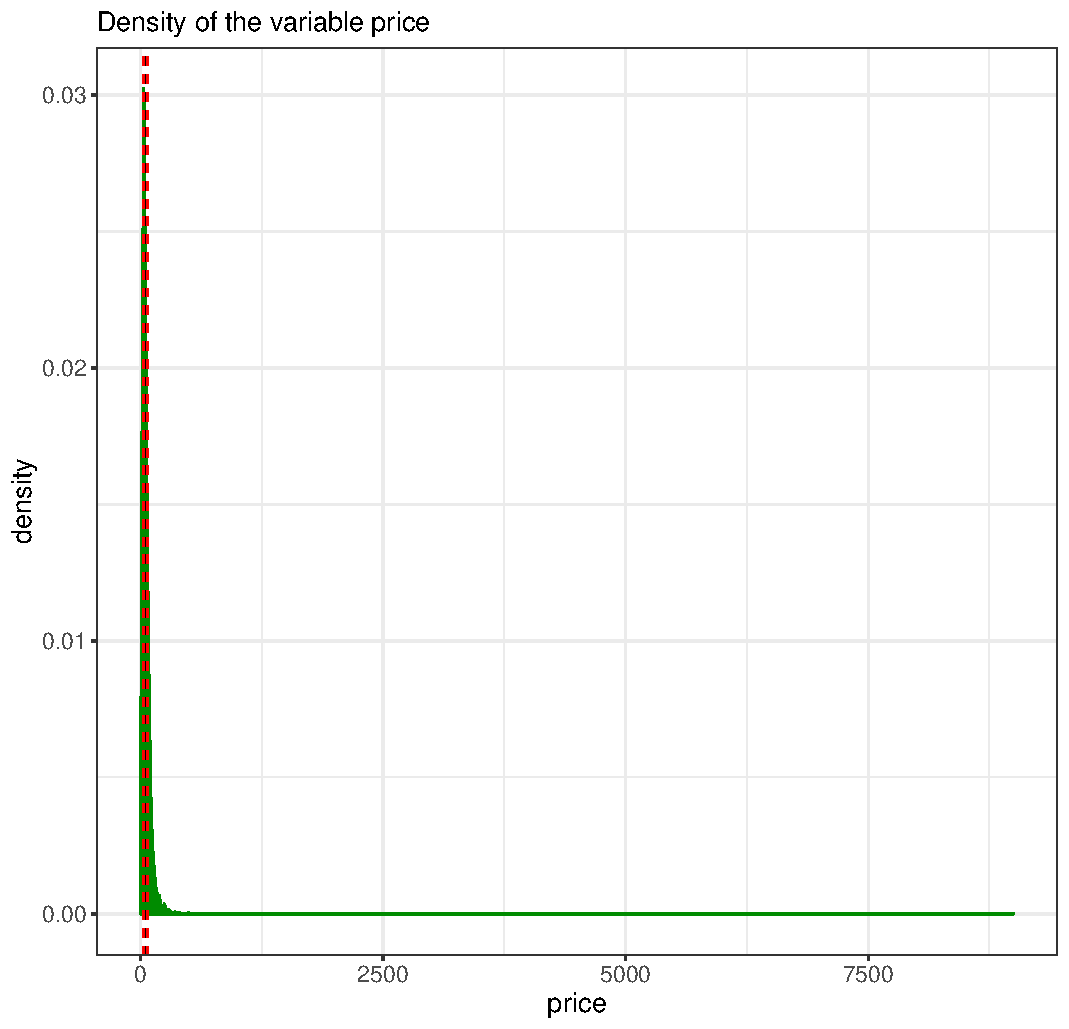
\includegraphics[height=7cm]{price_distribution_complete.pdf}}
\subfloat[Without outliers]{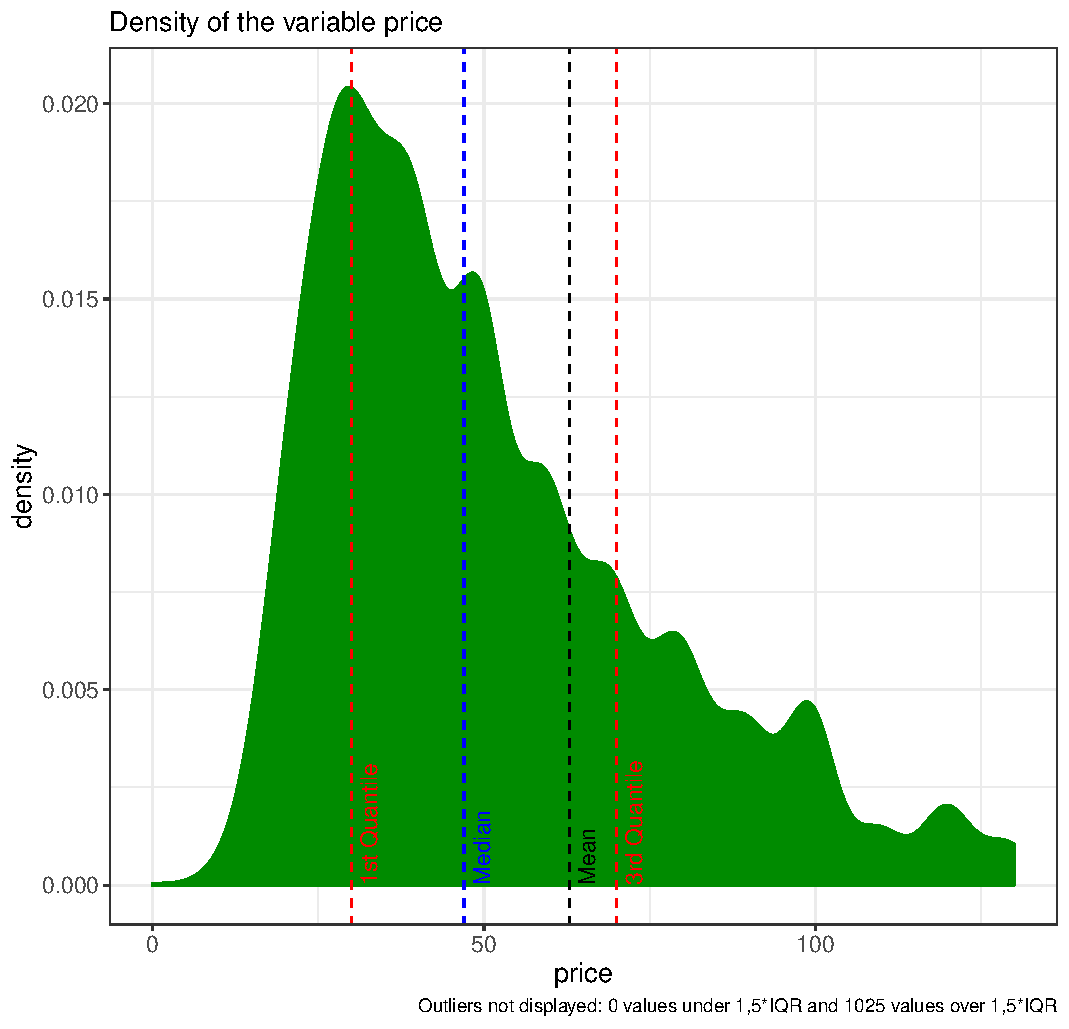
\includegraphics[height=7cm]{price_distribution_nooutliers.pdf}}
\caption{Distribution of the variable price \protect
\includegraphics[scale=0.05]{qletlogo.pdf} {\href{https://github.com/silvia-ventoruzzo/SPL-WISE-2018/blob/master/exploratory_data_analysis.R}{exploratory\_data\_analysis.R}}}
\centering
\end{figure}

For the categorical variables a bar plot is more appropriate, since the values that the variable can assume are discrete and usually also few, like in the case displayed in figure \ref{figure:room_type}.




\begin{figure}[H]
\begin{center}
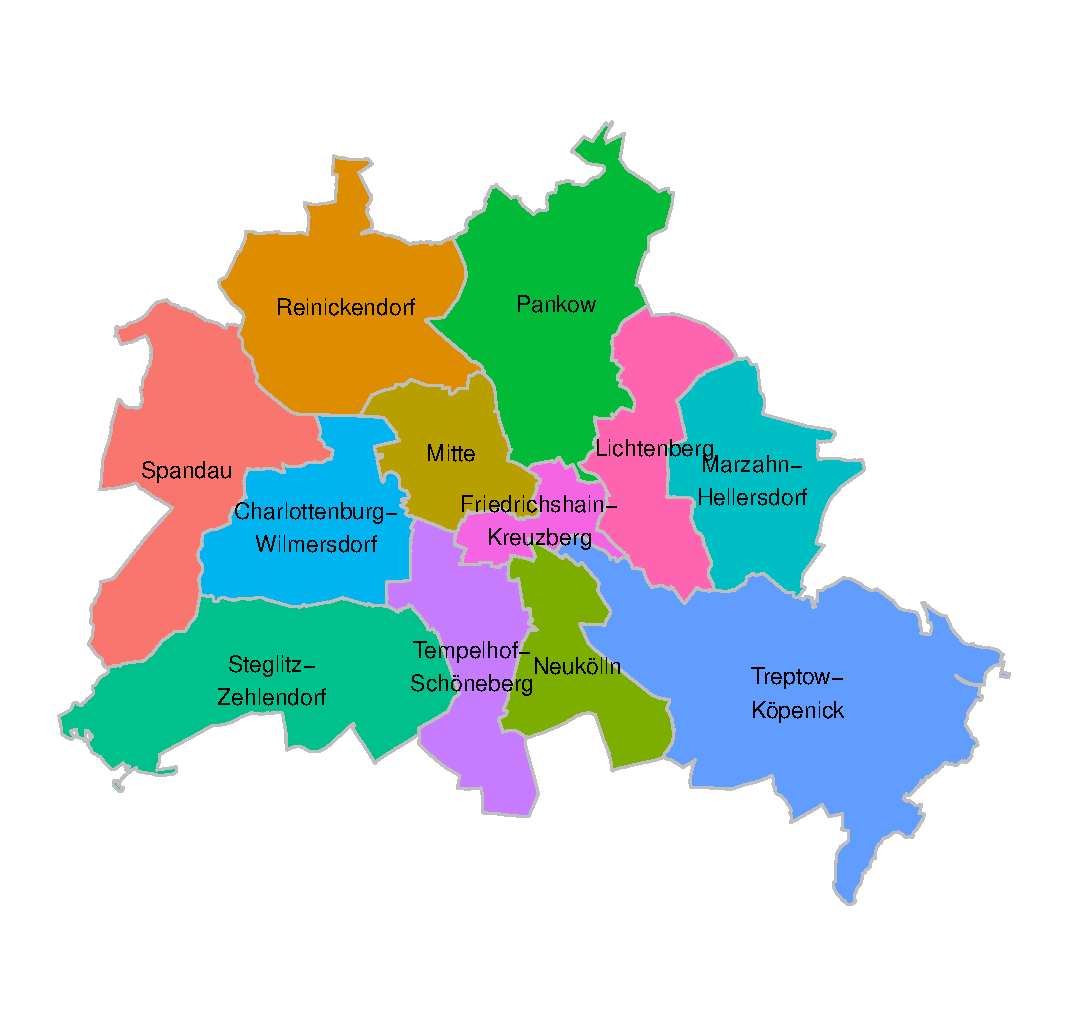
\includegraphics[width=0.5\textwidth, keepaspectratio]{room_type_distribution.pdf} \\
\caption{Distribution of the variable room\_type \protect
\includegraphics[scale=0.05]{qletlogo.pdf} {\href{https://github.com/silvia-ventoruzzo/SPL-WISE-2018/blob/master/exploratory_data_analysis.R}{exploratory\_data\_analysis.R}}}
\label{figure:room_type}
\end{center}
\end{figure}

We also mapped the Berlin districts and the distribution of the average of a certain variable on them with the use of the package \textit{leaflet}.

\begin{figure}[H]
\begin{center}
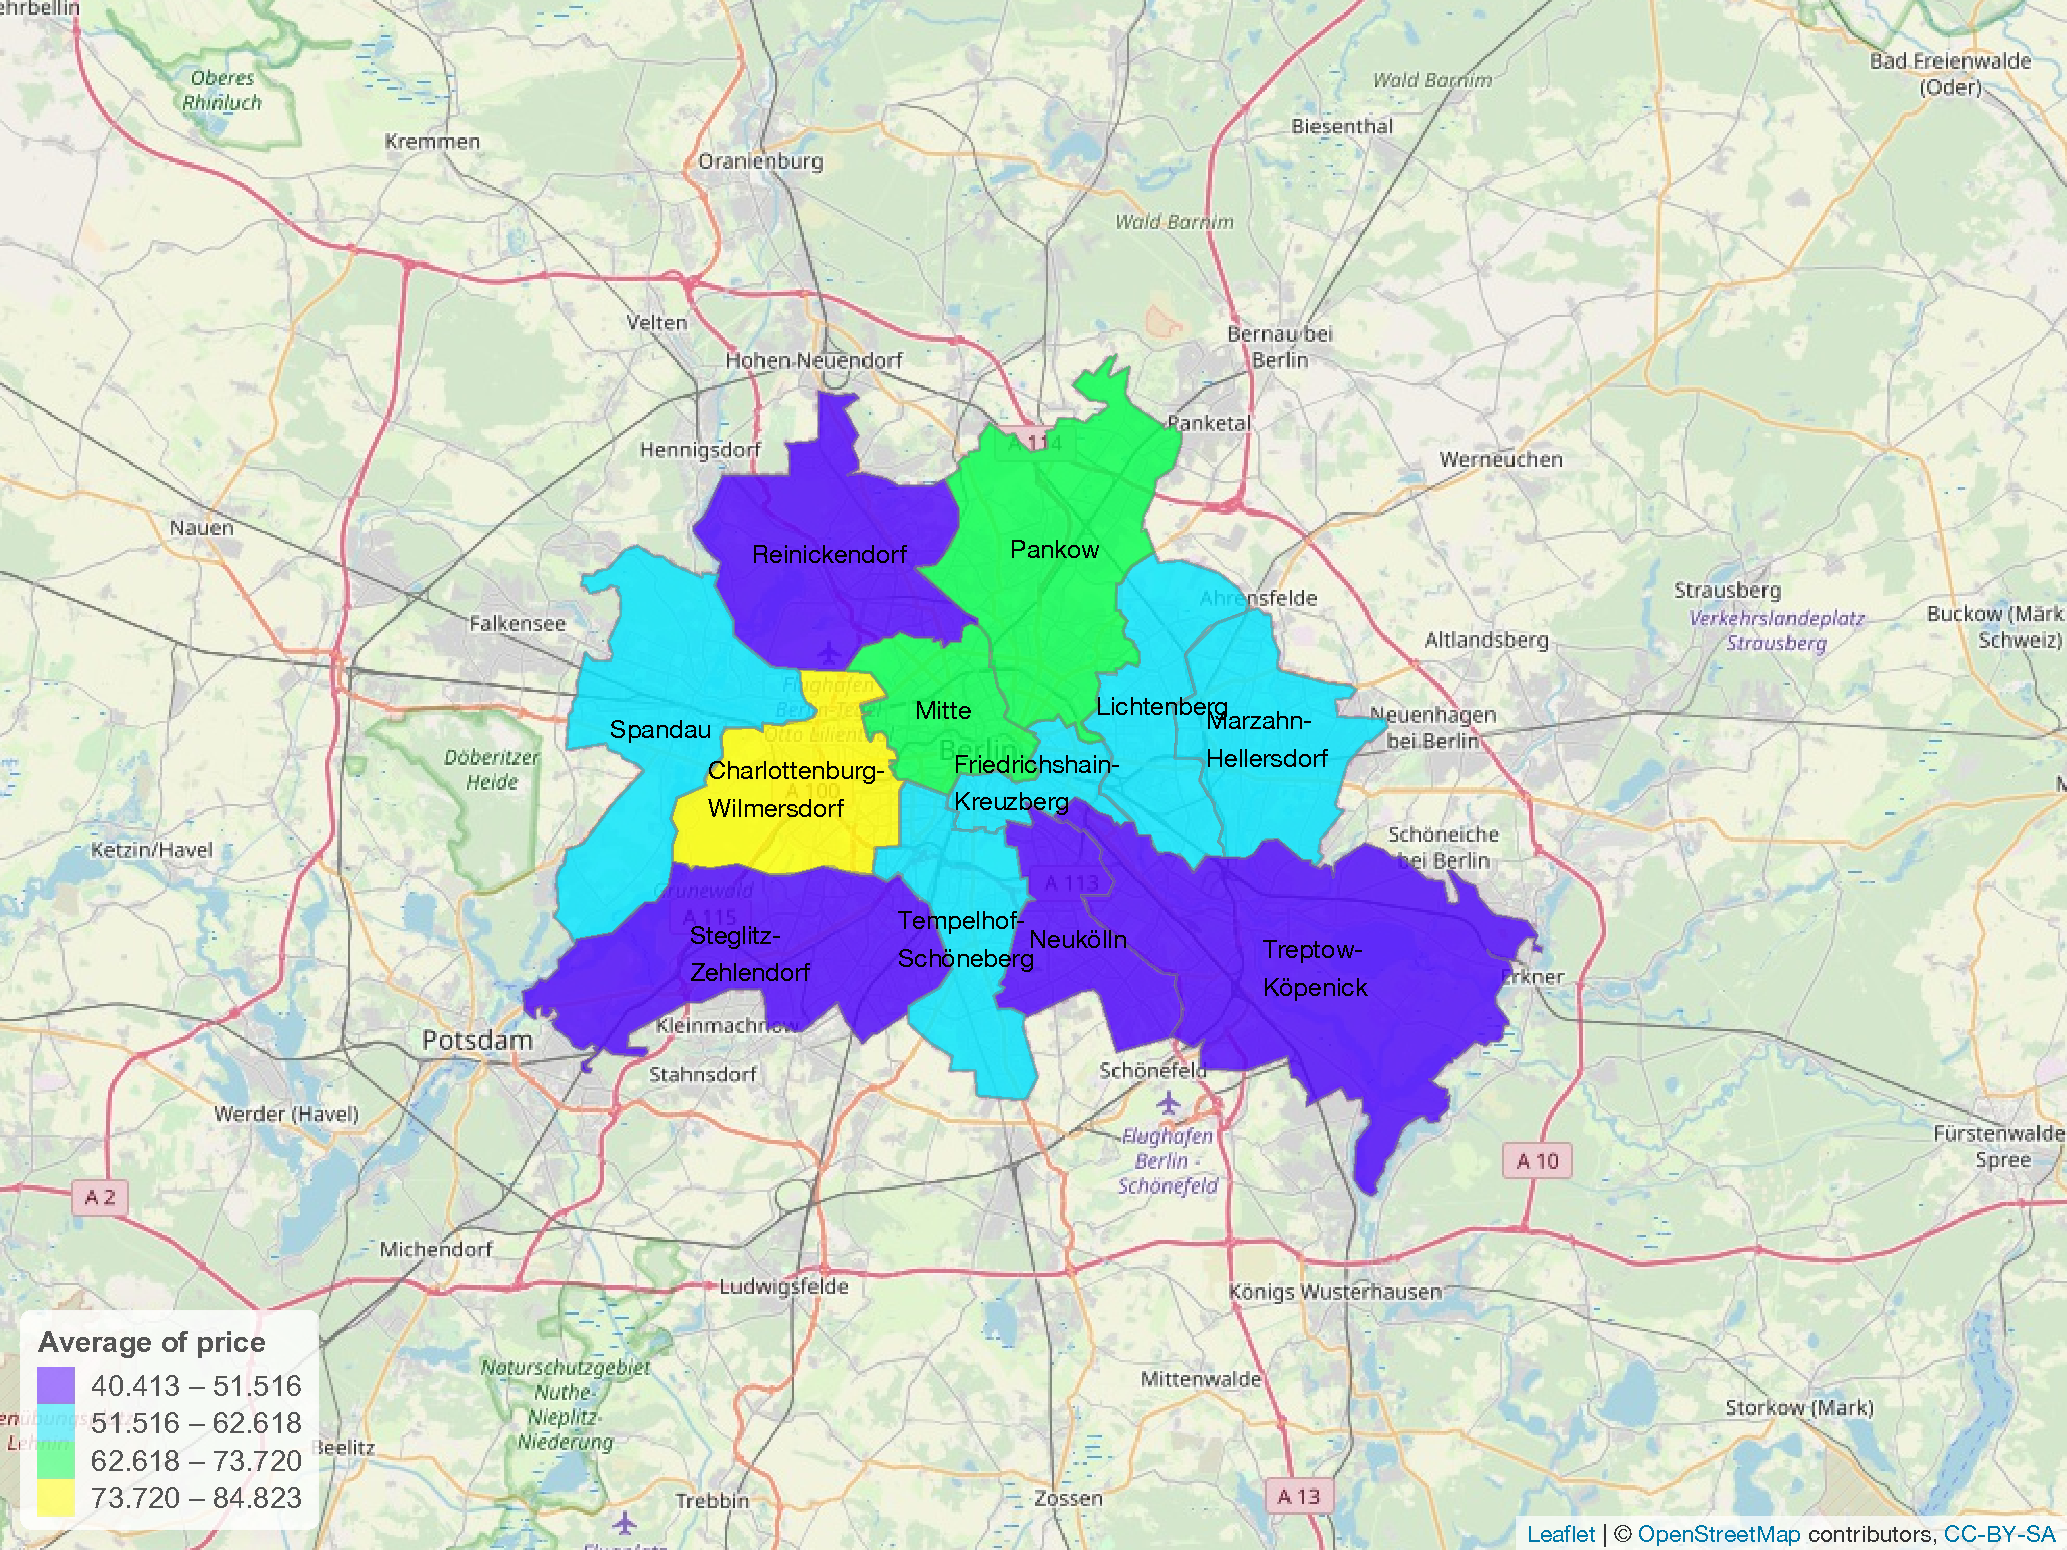
\includegraphics[width=0.5\textwidth, keepaspectratio]{price_map_distr} \\
\caption{Distribution of the average of price across Berlin's districts}
\label{figure:room_type}
\end{center}
\end{figure}